%From https://egu2018.eu/PICO_how-to_guide_to_PICO.pdf
%Abstracted and templated by Brian Ballsun-Stanton, Macquarie University.
%original template by https://github.com/snowtechblog/pico-latex-presentation by Anselm Köhler

\documentclass[unknownkeysallowed,usepdftitle=false, parskip=full]{beamer}
% unknownkeysallowed is needed for mac and the newer latex version -> is more picky than before...
\usetheme[headheight=1cm,footheight=2cm]{boxes}
%\usetheme{default}

\usefonttheme{serif}

\usepackage{default}
\usepackage{graphicx}
%example pictures created via: http://lorempixel.com/1200/800/cats/Figure2/. Credit to http://lorempixel.com/images.php

\usepackage{epsfig}
\usepackage{siunitx}
\usepackage{color}
\usepackage{ifthen}
%usepackage{ragged2e}sinuitsinsin


\usepackage[T1]{fontenc}
\usepackage[utf8]{inputenc}

%https://tex.stackexchange.com/a/203804/5483

\usepackage[activate={true,nocompatibility},final,tracking=true,kerning=true,spacing=true,factor=1100,stretch=10,shrink=10]{microtype} % http://www.khirevich.com/latex/microtype/
\microtypecontext{spacing=nonfrench}

\usepackage{lipsum} % for dummy text only
\usepackage[UKenglish]{babel} %https://tex.stackexchange.com/a/27743 
\usepackage[pangram]{blindtext} % https://tex.stackexchange.com/a/48411

%\usepackage{parskip} % from https://tex.stackexchange.com/q/11622
%\setlength{\parskip}{12pt} 

%\setparsizes{\parindent}{12pt}{\parfillskip}

%\usepackage{etoolbox} % as per https://tex.stackexchange.com/a/24331
%\appto\chapterheadendvskip{\vspace{-1\parskip}}
%\setparsizes{\parindent}{50pt plus 20pt minus 30pt}{\parfillskip}

\setbeamertemplate{navigation symbols}{}%remove navigation symbols
\setbeamersize{text margin left=1cm,text margin right=1cm}

% some colors
\definecolor{grau}{gray}{.5}
\definecolor{slfcolor}{RGB}{187,85,237}
\definecolor{wslcolor}{RGB}{242,114,137}
\definecolor{buttons}{RGB}{157, 218, 245}

% setup links
\hypersetup{%
	%linkbordercolor=green,%
	colorlinks=false,%
	pdfborderstyle={/S/U/W 0},%
	%pdfpagemode=FullScreen,%
	pdfstartpage=4,%
	}

% setup some fonts
\setbeamerfont{title}{series=\bfseries, size=\large}
\setbeamerfont{author}{size*={7pt}{0pt}}
\setbeamerfont{institute}{size*={3pt}{0pt}}
\setbeamerfont{bodytext}{size=\scriptsize}
	
% Title setup	
\title{IMPROVING THE WRITING AND ORGANISING OF NOTES ON A FILM}
\author{Emily Hunt \texttt{emily.hunt@students.mq.edu.au}}
% add title in headbox
\setbeamertemplate{headline}
{\leavevmode
\begin{beamercolorbox}[width=1\paperwidth]{head title}
  % LOGO
   \centering \usebeamerfont{title} \textcolor{slfcolor}{\inserttitle} \\
   \vspace{0.15cm}
   \centering \usebeamerfont{author} \color[rgb]{0,0,0} \insertauthor \\
   \vspace{0.1cm}
   \centering \usebeamerfont{institute} \insertinstitute
 
  {\color{slfcolor}\hrule height 1pt\vspace{0.1cm}}
\end{beamercolorbox}%
}

% setup the navigation in footbox
% first set some button colors
\newcommand{\buttonactive}{\setbeamercolor{button}{bg=wslcolor,fg=white}}
\newcommand{\buttonpassive}{\setbeamercolor{button}{bg=buttons,fg=black}}
% now set up that the one active one gets the new color.
\newcommand{\secvariable}{nothing}
% therefore we write before each section (well, everything which should be part of the navi bar)
% the variable \secvariable to any name which is in the next function ...
\newcommand{\mysection}[1]{\renewcommand{\secvariable}{#1}
}
% ... compaired to strings in the following navibar definition ...
\newcommand{\tocbuttoncolor}[1]{%
 \ifthenelse{\equal{\secvariable}{#1}}{%
    \buttonactive}{%
    \buttonpassive}
 }
% ... here we start to set up the navibar. each entry is calling first the function \tocbuttoncolor with the argument which should be tested for beeing active. if active, then change color. afterwards the button is draw. so to change that, you need to change the argument in \toc..color, the first in \hyperlink and before each frames definition... A bit messed up, but works...
\newlength{\buttonspacingfootline}
\setlength{\buttonspacingfootline}{-0.2cm}
\setbeamertemplate{footline}
{\leavevmode
\begin{beamercolorbox}[width=1\paperwidth]{head title}
  {\color{slfcolor}\hrule height 1pt}
  \vspace{0.05cm}
  % set up the buttons in an mbox
  \centering \mbox{
    \tocbuttoncolor{abstract}
    \hyperlink{abstract}{\beamerbutton{2 Minute Madness}}
    \tocbuttoncolor{radar}
    \hspace{\buttonspacingfootline}
      \hyperlink{radar}{\beamerbutton{oTranscribe}}

    \tocbuttoncolor{line}
    \hspace{\buttonspacingfootline}
      \hyperlink{line}{\beamerbutton{Shell Script}}
    \tocbuttoncolor{major}
    \hspace{\buttonspacingfootline}
      \hyperlink{major}{\beamerbutton{Testing}}
    \tocbuttoncolor{slab}
    \hspace{\buttonspacingfootline}
      \hyperlink{slab}{\beamerbutton{Results}}
    \tocbuttoncolor{minor}
    \tocbuttoncolor{conclusion}
    \hspace{\buttonspacingfootline}
      \hyperlink{conclusion}{\beamerbutton{Conclusion}}
    % this last one should normaly not be used... it will open the preferences to change the 
    % behaviour of the acrobat reader in fullscreen -> usefull in pico...
    \setbeamercolor{button}{bg=white,fg=black}
    % for presentation
    %\hspace{-0.1cm}\Acrobatmenu{FullScreenPrefs}{\beamerbutton{\#}}
    % for upload
    
     
\Acrobatmenu{FullScreenPrefs}{\vspace{0.3cm}\hspace{0.24cm}\mbox{%
      
\includegraphics[height=0.04\textheight,keepaspectratio]{%
	  figure/CreativeCommons_Attribution_License.eps}%
	  }}
   }
    \vspace{0.05cm}
\end{beamercolorbox}%
}


\begin{document}


%%%%%%%%%%%%%%%%%%%%%%%%%%%%%%%%%%%%%%%%%%%%%%%%%%%%%%%%%%%%%%%%%%%%%%%%%%
\mysection{abstract}
%%%%%%%%%%%%%%%%%%%%%%%%%%%%%%%%%%%%%%%%%%%%%%%%%%%%%%%%%%%%%%%%%%%%%%%%%%
\begin{frame}\label{\secvariable}

 \begin{columns}[t]
  %https://tex.stackexchange.com/a/7452/5483
  
      \begin{column}[c]{0.45\textwidth}
    \parbox{\linewidth}{
    
    \textbf{The Problem}

\vspace{1pt}

      When taking notes on a film:  
      
      \vspace{1pt}
      
      \begin{itemize}
          \item I would provide no concrete indication of what point of the film I was referring to, requiring me to scrub through to find it.
      \end{itemize}
      \begin{itemize}
          \item I would spend a lot of time searching my notes for observations on particular ideas (e.g. the use of colour).
      \end{itemize}
      }
    \end{column}
  
  \begin{column}[c]{0.45\textwidth}
%http://lorempixel.com/1200/800/cats/Figure2/     
%http://lorempixel.com/1200/800/cats/Figure3/
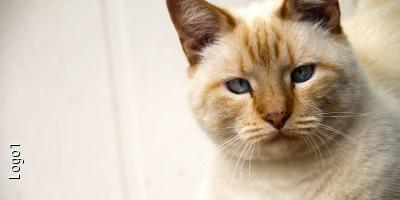
\includegraphics[width=1\textwidth,height=0.5\textheight,keepaspectratio]{%
figure/logo1.png}\\
\tiny{This is a small caption}

\vspace{20pt}
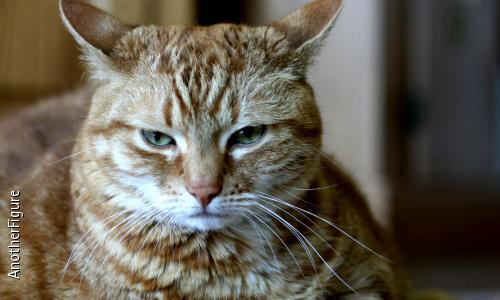
\includegraphics[width=1\textwidth,height=0.5\textheight,keepaspectratio]{%
figure/figure1.png}

\tiny{This is a small caption}
    \end{column}
    
  \end{columns}

  

   
\end{frame}

\begin{frame}\label{\secvariable}
  \begin{columns}[t]
  %https://tex.stackexchange.com/a/7452/5483
  \begin{column}[c]{0.45\textwidth}
%http://lorempixel.com/1200/800/cats/Figure2/     
%http://lorempixel.com/1200/800/cats/Figure3/
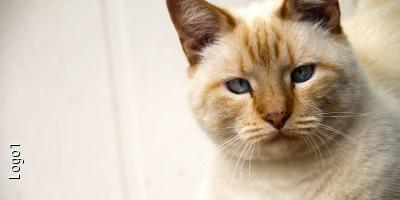
\includegraphics[width=1\textwidth,height=0.5\textheight,keepaspectratio]{%
figure/logo1.png}\\
\tiny{This is a small caption}

\vspace{12pt}
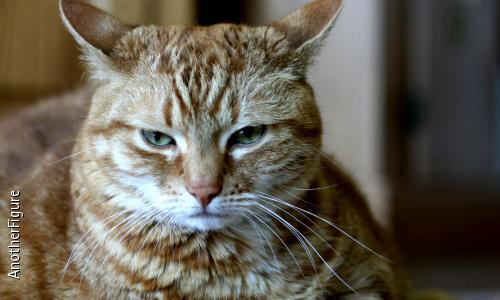
\includegraphics[width=1\textwidth,height=0.5\textheight,keepaspectratio]{%
figure/figure1.png}

\tiny{This is a small caption}
    \end{column}
    \begin{column}[c]{0.45\textwidth}
    \parbox{\linewidth}{
    
        \textbf{The Solution}

\vspace{1pt}

      \begin{itemize}
          \item \small{oTranscribe -- \textgreater{} allows you to take notes while watching a video with a timestamp. I am running the software myself on GitHub, ensuring its availability.}
      \end{itemize}
      \begin{itemize}
          \item \small{A shell script to sort notes exported from oTranscribe into separate files based on their mention of the keywords: camera, character, colour, editing, lighting, narrative, sound, and/or theme.}
      \end{itemize}
      }
    \end{column}
    
  \end{columns}

  
\end{frame}

%%%%%%%%%%%%%%%%%%%%%%%%%%%%%%%%%%%%%%%%%%%%%%%%%%%%%%%%%%%%%%%%%%%%%%%%%%
\mysection{radar}
%%%%%%%%%%%%%%%%%%%%%%%%%%%%%%%%%%%%%%%%%%%%%%%%%%%%%%%%%%%%%%%%%%%%%%%%%%
\begin{frame}\label{\secvariable}
  
\textbf{Steps to Run oTranscribe}

\begin{itemize}
   \item I downloaded oTranscribe's \href{https://github.com/oTranscribe/oTranscribe}{GitHub Repository}.
   \item Using the files downloaded from the repositoy, I compiled a dist folder using NPM and Node.js.
   \item I installed Jekyll.
   \item I copied the contents of the complied dist folder to a folder called docs and pushed this to my Hunt-Exercises repository on GitHub.
   \item I created index.md in my repository and within this file, created a link to the docs folder. I then selected that GitHub paes run off the master branch of by repository.
   \item This can be accessed with my entire proof of concept at \url{https://mq-foar705.github.io/Hunt-Exercises/}
\end{itemize}  
      
      \hyperlink{oTranscribe_interface}{\beamerbutton{oTranscribe Interface}}\\

\end{frame}

\begin{frame}\label{\secvariable}
\label{oTranscribe_interface}
\hyperlink{slab}{\beamerbutton{\dots back to steps}}\\
\begin{center}
  \vspace{-0.2cm}
  %http://lorempixel.com/1200/800/cats/Figure4/
 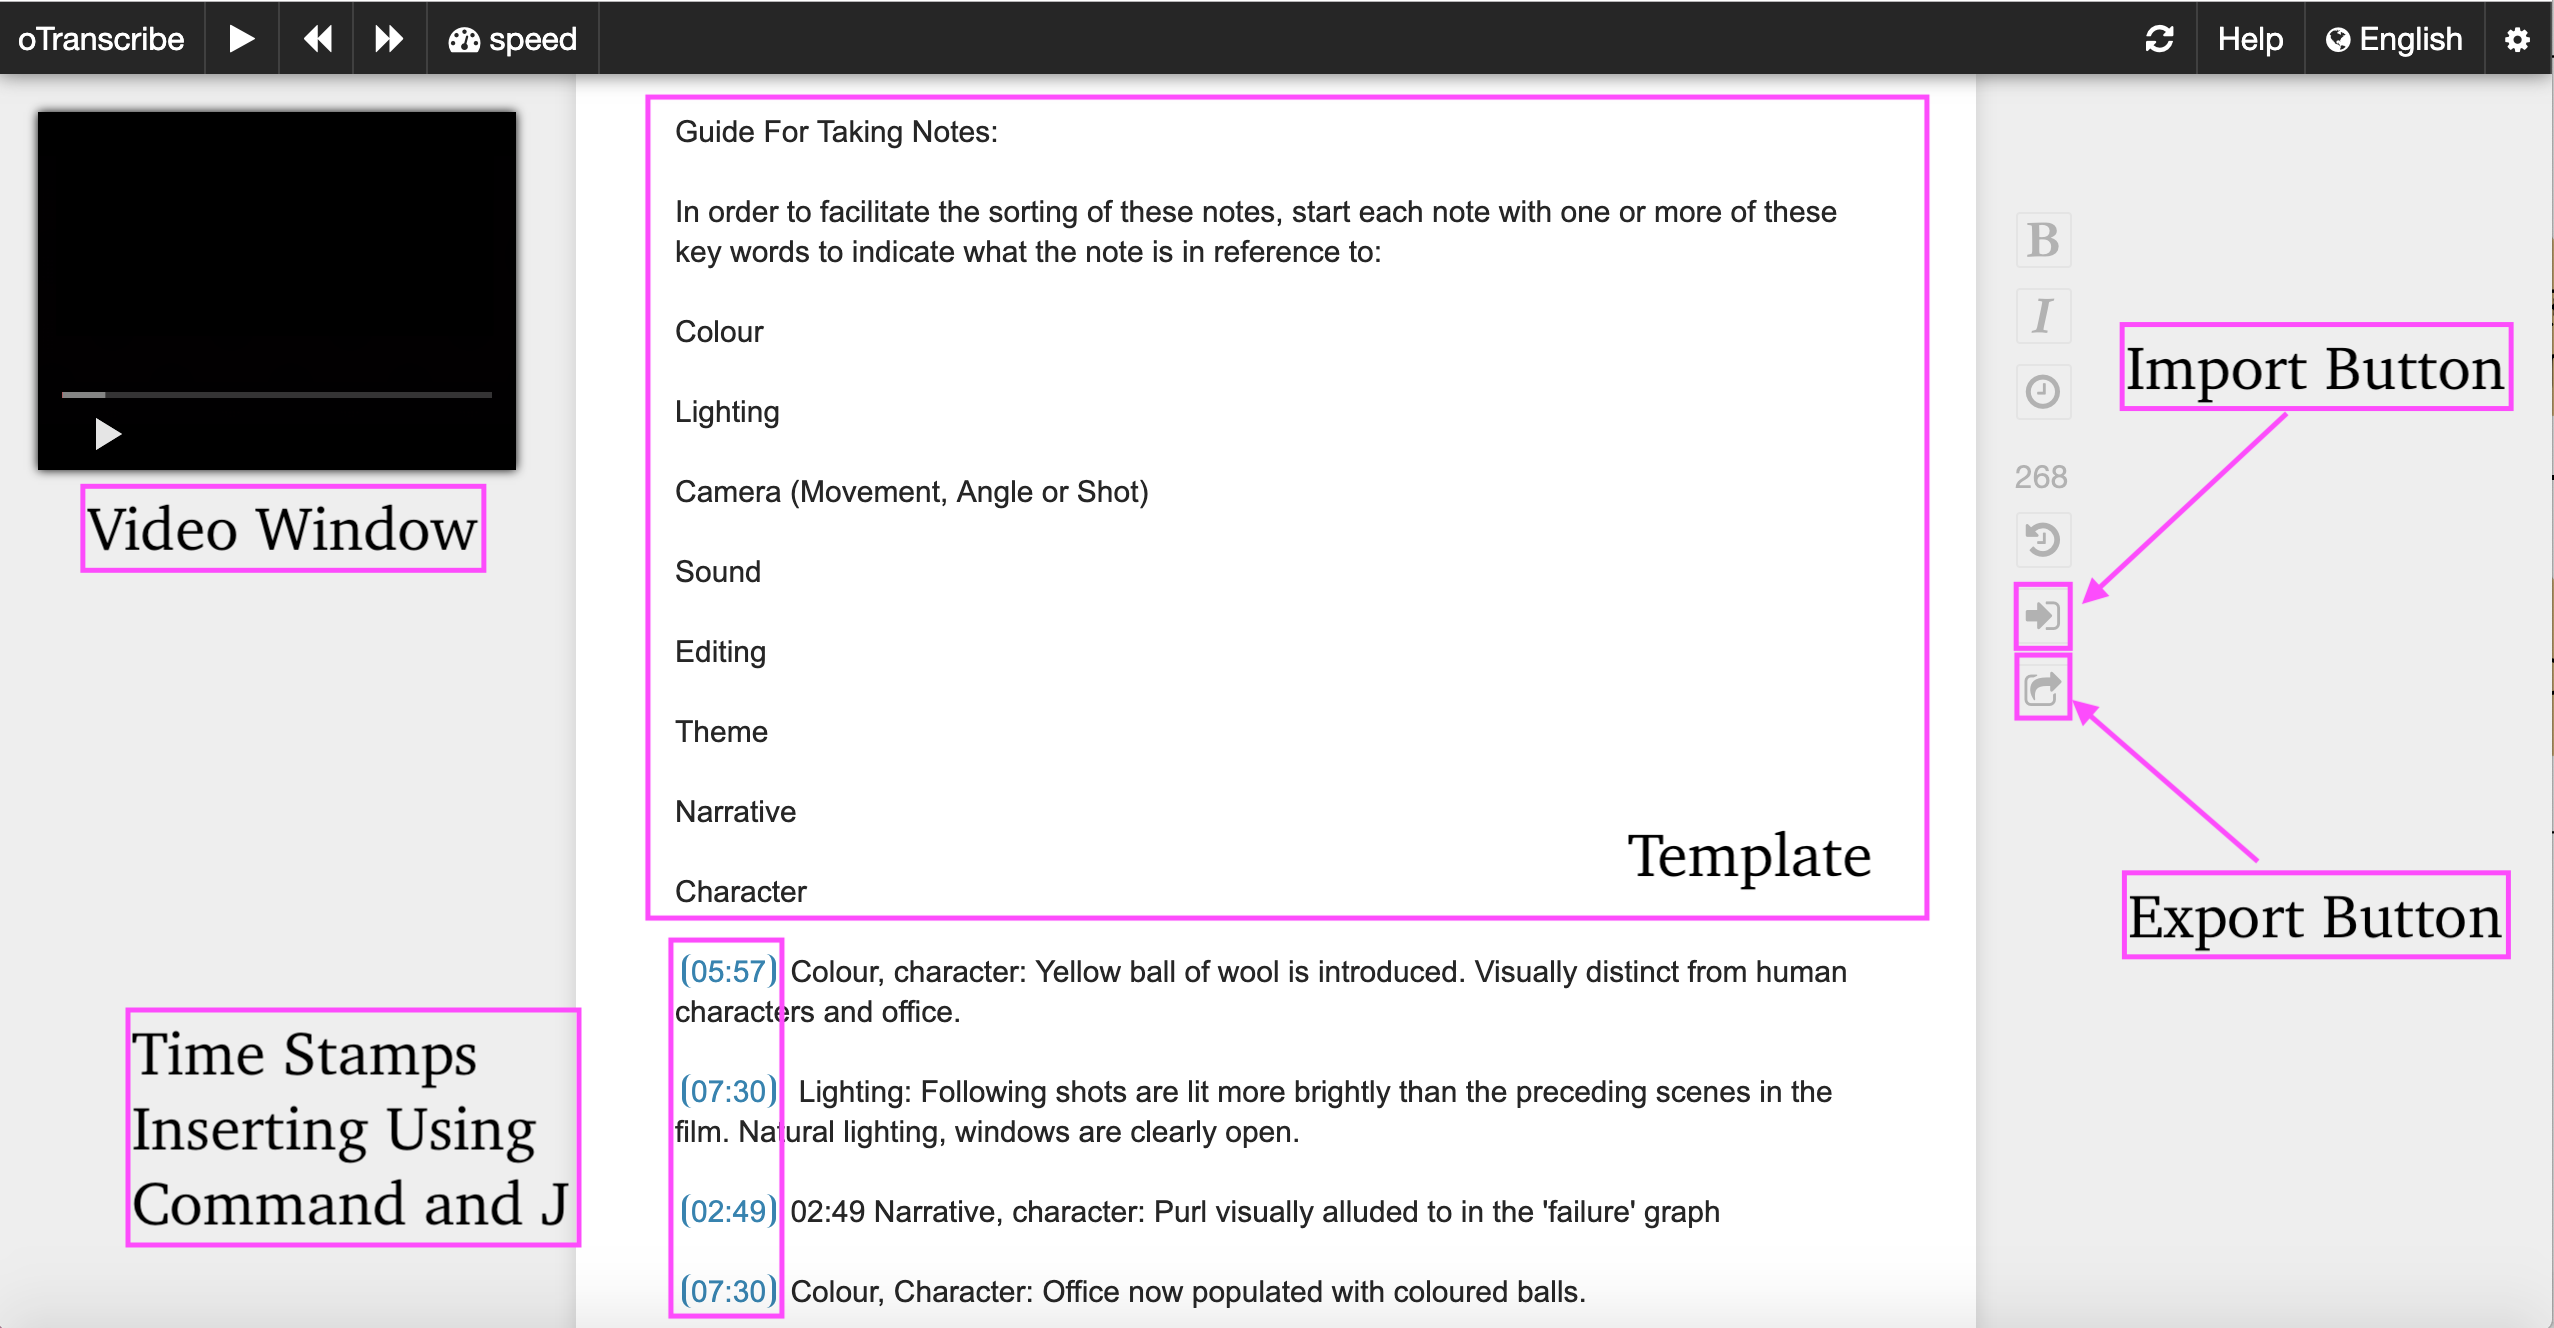
\includegraphics[width=1\textwidth,height=1\textheight,keepaspectratio]{%
  figure/oTranscribe_labels.png}
\end{center}
\end{frame}

%%%%%%%%%%%%%%%%%%%%%%%%%%%%%%%%%%%%%%%%%%%%%%%%%%%%%%%%%%%%%%%%%%%%%%%%%%
\mysection{line}
%%%%%%%%%%%%%%%%%%%%%%%%%%%%%%%%%%%%%%%%%%%%%%%%%%%%%%%%%%%%%%%%%%%%%%%%%%
\begin{frame}\label{\secvariable}
\begin{center}
  \vspace{-0.5cm}
\textbf{Shell Script}\\
\vspace{2pt}
\footnotesize{The below right is my shell script to sort a txt file exported from oTranscribe into eight separate txt files based on their mention of keywords.\\
With the Film Name folder in a directory set up like the one in the image on the below left, run} \\
\texttt{bash code/organise\textunderscore notes.sh data/Film\textunderscore Notes.txt}

\end{center}

 \begin{columns}[t]
  %https://tex.stackexchange.com/a/7452/5483
  
      \begin{column}[c]{0.45\textwidth}

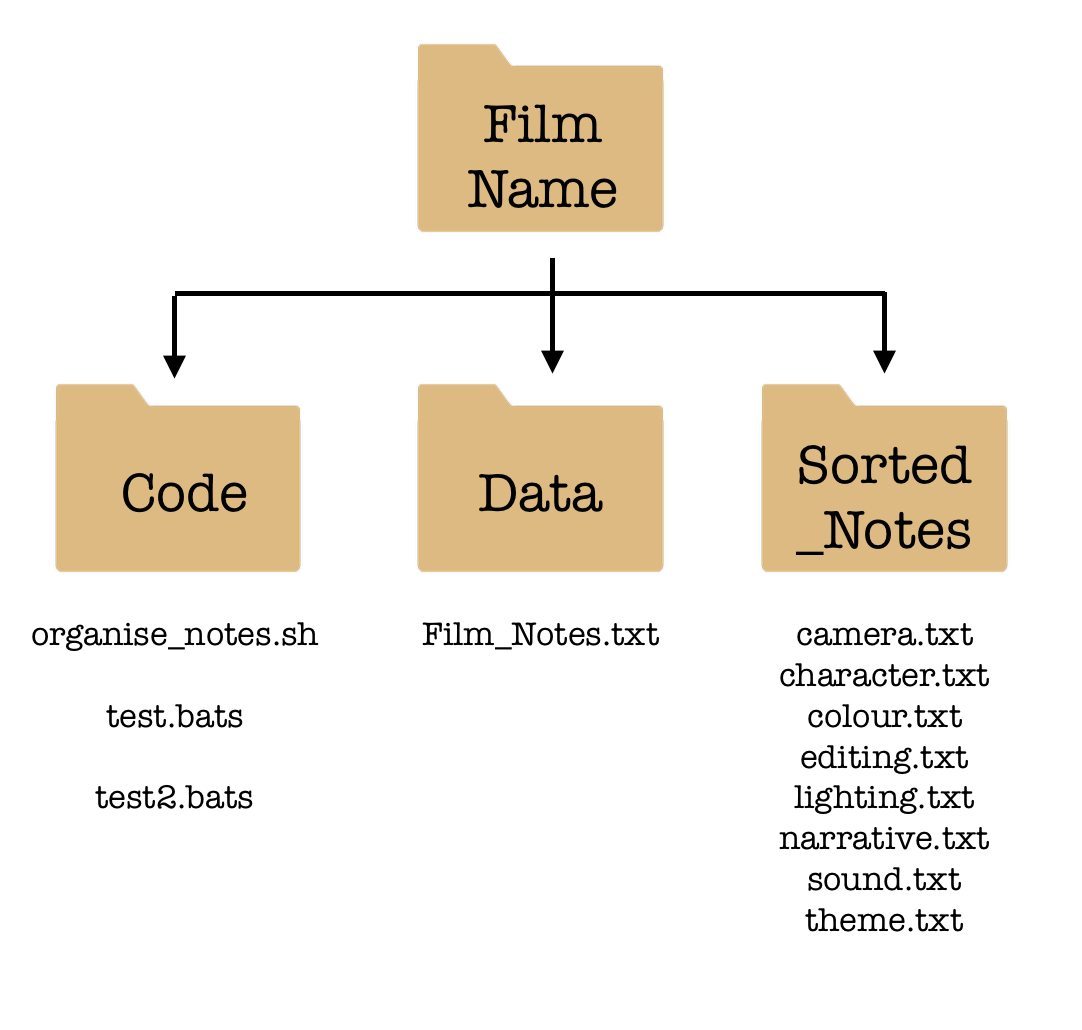
\includegraphics[width=1\textwidth,height=2\textheight,keepaspectratio]{%
figure/directory_structure.png}

    \end{column}
  
  \begin{column}[c]{0.45\textwidth}

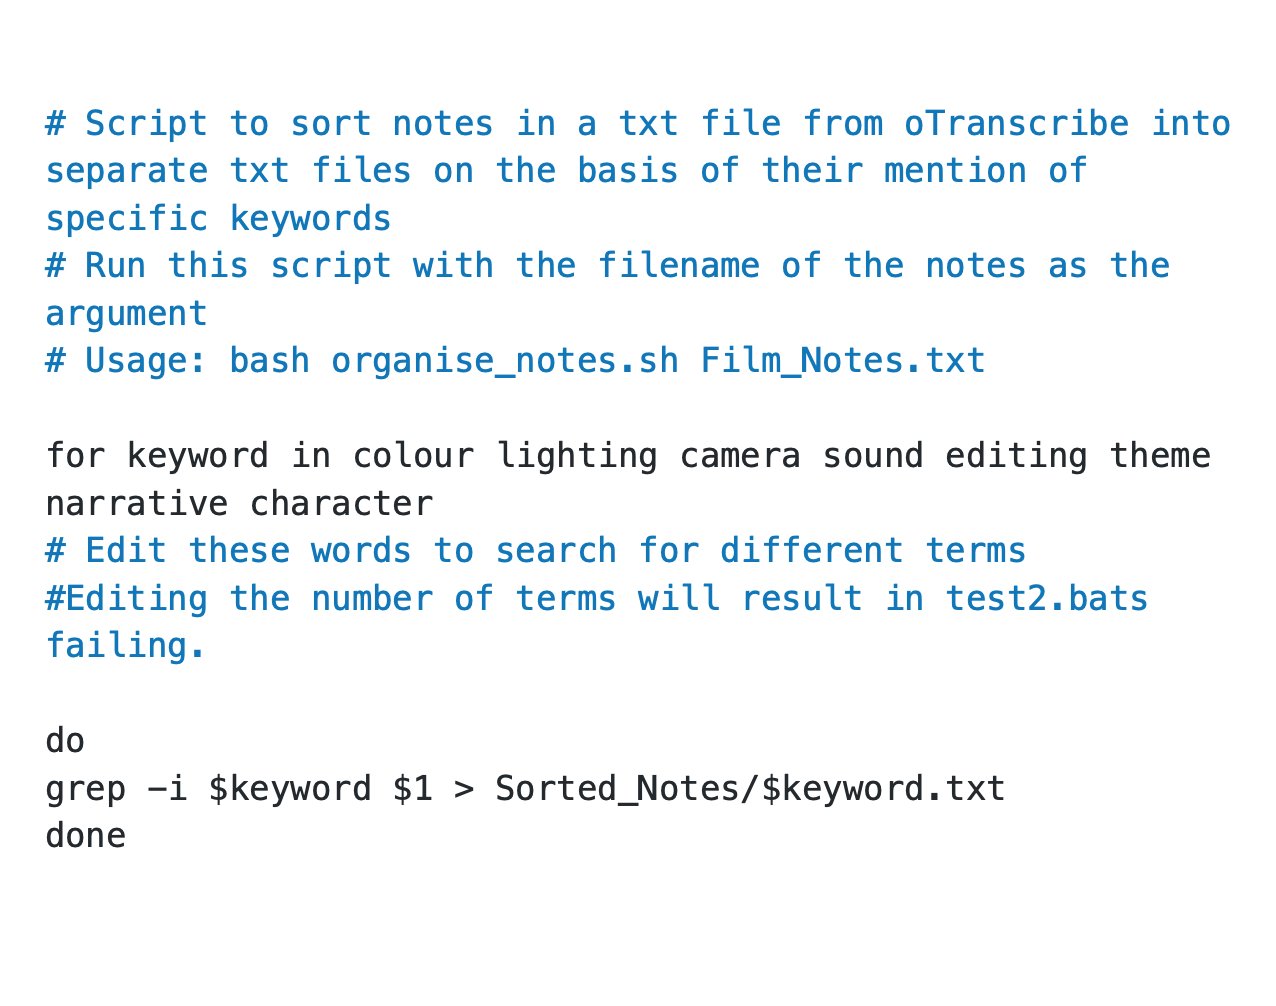
\includegraphics[width=1\textwidth,height=0.5\textheight,keepaspectratio]{%
figure/shell_script.png}



    \end{column}
    
    
  \end{columns}

\begin{center}
Creative commons attribution    
\end{center}

  
\end{frame}

%%%%%%%%%%%%%%%%%%%%%%%%%%%%%%%%%%%%%%%%%%%%%%%%%%%%%%%%%%%%%%%%%%%%%%%%%%
\mysection{major}
%%%%%%%%%%%%%%%%%%%%%%%%%%%%%%%%%%%%%%%%%%%%%%%%%%%%%%%%%%%%%%%%%%%%%%%%%%
\begin{frame}\label{\secvariable} %%Eine Folie
 \begin{columns}[t]
  %https://tex.stackexchange.com/a/7452/5483
  
 
  
      \begin{column}[c]{0.45\textwidth}
    {
    
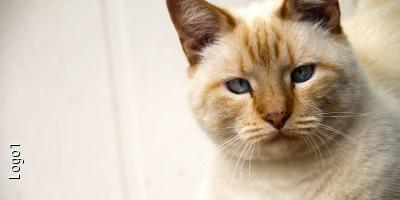
\includegraphics[width=1\textwidth,height=0.5\textheight]{%
figure/logo1.png}\\

\vspace{20pt}

\begin{center}

This test was designed to ensure

\end{center}

      }
    \end{column}
  
  \begin{column}[c]{0.45\textwidth}

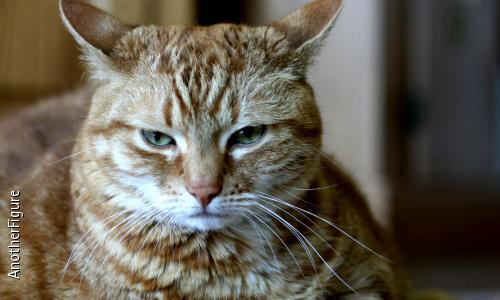
\includegraphics[width=1\textwidth,height=0.5\textheight]{%
figure/figure1.png}

\vspace{20pt}

\begin{center}

This test was designed to ensure

\end{center}
      
    \end{column}
    
  \end{columns}
\end{frame}

%%%%%%%%%%%%%%%%%%%%%%%%%%%%%%%%%%%%%%%%%%%%%%%%%%%%%%%%%%%%%%%%%%%%%%%%%%
\mysection{slab}
%%%%%%%%%%%%%%%%%%%%%%%%%%%%%%%%%%%%%%%%%%%%%%%%%%%%%%%%%%%%%%%%%%%%%%%%%%
\begin{frame}\label{\secvariable}
%http://lorempixel.com/1200/800/cats/Figure6/
\begin{center}
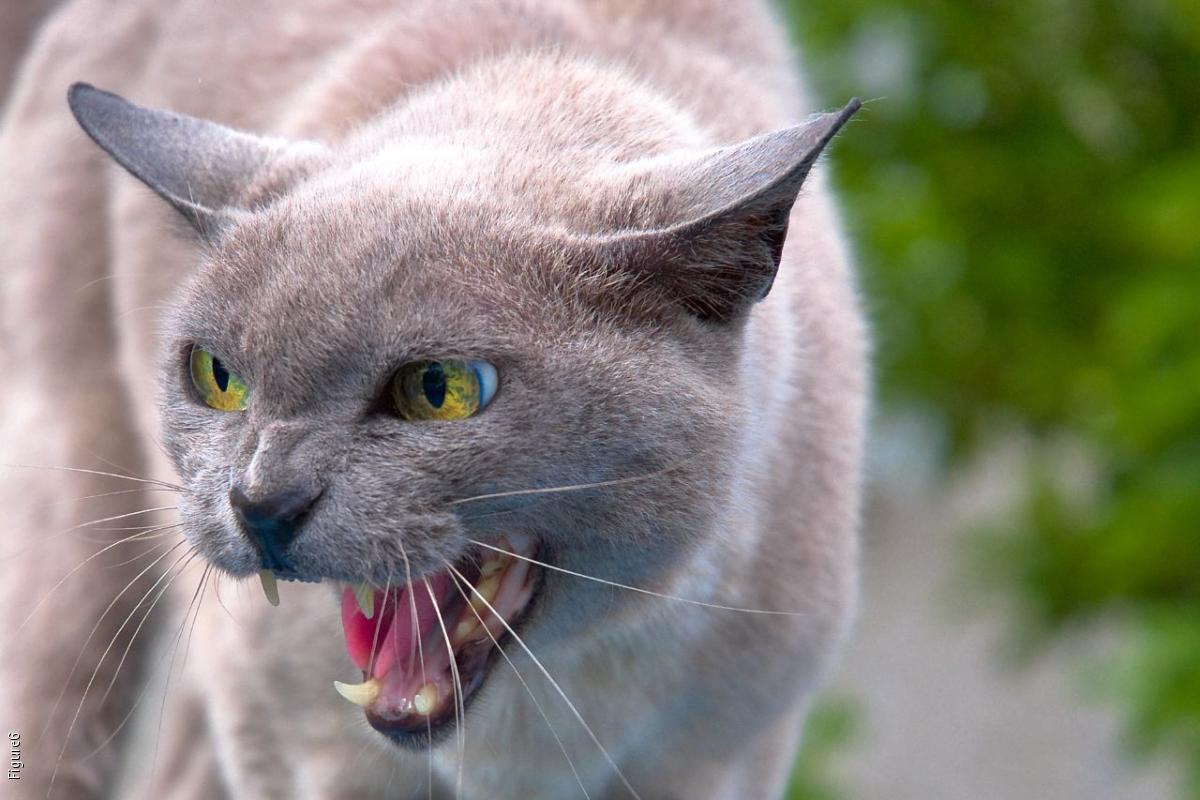
\includegraphics[width=1\textwidth,height=0.75\textheight,keepaspectratio]{%
figure/figure6.png}
\end{center}
    \parbox{\linewidth}{

Etiam cursus nibh nec ex tincidunt pharetra quis vel nibh. Sed condimentum lobortis mollis. Donec vitae odio nec lacus iaculis condimentum. Proin dictum consequat quam nec. }

\end{frame}


%%%%%%%%%%%%%%%%%%%%%%%%%%%%%%%%%%%%%%%%%%%%%%%%%%%%%%%%%%%%%%%%%%%%%%%%%%
\mysection{conclusion}
%%%%%%%%%%%%%%%%%%%%%%%%%%%%%%%%%%%%%%%%%%%%%%%%%%%%%%%%%%%%%%%%%%%%%%%%%%
\begin{frame}\label{\secvariable}
  
  \begin{itemize}
   \item Curabitur viverra massa vel elit tincidunt lacinia. Pellentesque id est lobortis, interdum felis nec, faucibus augue. Suspendisse varius sit amet dui ac dignissim. Quisque mattis, odio a congue lobortis, eros turpis placerat enim, ac tempor lorem nisl ut velit. Mauris vel nulla a quam viverra faucibus. 
  \item Quisque sed orci eu libero mattis lobortis. Curabitur aliquam lorem neque, ac auctor justo sagittis sed. Nunc augue nisl, mattis sed turpis at, elementum lobortis augue. Vestibulum porta felis bibendum mattis iaculis. Nulla dignissim varius rutrum.
  \item Vivamus eget semper nunc. Donec sodales ornare porttitor. Curabitur commodo viverra arcu. Aliquam consequat felis non dolor consequat ultricies. Mauris non finibus nisl. Sed tincidunt felis at porttitor posuere.

  \end{itemize}

  \usebeamerfont{bodytext}
  K\"ohler, A., J. N. McElwaine, B. Sovilla, M. Ash, P. Brennan (in Review),
Surge dynamics of the 3 February 2015 avalanches in Valle\'e de la Sionne,
\textit{J. Geophys. Res.} 
  
\end{frame}




\end{document}
